\section{Modularity}
\label{sec:modularity}

Since the framework developed in the course of this thesis is required to be highly modular, we first need to define the term \textit{Modularity}, find out how it relates to software engineering and choose a tool for supporting modularity on the Java platform.

Modularity is a frequently used term in Software Engineering. To understand the fundamental concept of it, take a look at the following definitions:

\begin{quote}
Large software systems are inherently more complex to develop and maintain than smaller systems. Modularity involves breaking a large system into separate physical entities that ultimately makes the system easier to understand.

\hfill \textbf{Java Application Architecture}

\hfill \citeauthor{Knoernschild:2012} \cite{Knoernschild:2012}
\end{quote}

\begin{quote}
Systems are deemed “modular” when they can be decomposed into a number of components. The components are able to connect, interact, or exchange resources in some way, by adhering to a standardized interface. Unlike a tightly integrated product whereby each component is designed to work specifically with other particular components in a tightly coupled system, modular products are systems of components that are loosely coupled.

\hfill \textbf{Modularity}

\hfill \citeauthor{Wikipedia:Modularity:2012} \cite{Wikipedia:Modularity:2012}
\end{quote}

Basically, modularity is based on modules, their requirements and behaviour. To fully understand the meaning of modularity we need to focus on the \textit{module} itself:

\subsection{Module definition}
\label{sec:module}

According to \citeauthor{Knoernschild:2012}, a software module is defined as follows:

\begin{quote}
A software module is a deployable, manageable, natively reusable, composable, stateless unit of software that provides a concise interface to consumers. 

\hfill \textbf{Java Application Architecture}

\hfill \citeauthor{Knoernschild:2012} \cite{Knoernschild:2012}
\end{quote}

\begin{figure}[H]
\centering
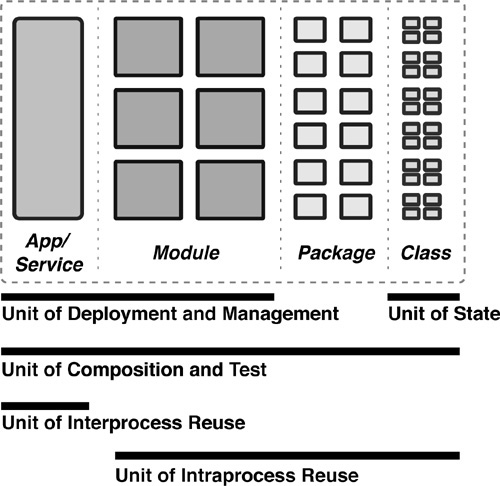
\includegraphics[width=0.8\textwidth]{module.jpeg}
\caption{Module definition diagram}
\label{fig:module}
\end{figure}

Figure \ref{fig:module} illustrates this defnition and all the individual aspects of a module \cite{Knoernschild:2012}:

\subsection{OSGi}
\gls{OSGi} is the most widely used and highly developed module system and service platform for the Java environment. This chapter aims to show why \gls{OSGi} is the best choice for building highly modular Java-based software systems as it supports all requirements of modularity defined by \citeauthor{Knoernschild:2012}\cite{Knoernschild:2012}.

The \gls{OSGi} technology is a set of specifications that define a dynamic component system for Java. These specifications enable a development model where applications are dynamically composed of many different reusable components. The \gls{OSGi} specifications enable modules to hide their implementations from other modules while communicating through services, which are objects that are specifically shared between modules. This surprisingly simple model has far reaching effects for almost any aspect of the software development process \cite{OSGi}. In \gls{OSGi} parlance, a module is known as a bundle. \gls{OSGi} provides a framework for managing bundles that are packaged as regular Java JAR files with an accompanying manifest. The manifest contains important metadata that describes the bundles and its dependencies to the \gls{OSGi} framework \cite{Knoernschild:2012}. Figure \ref{fig:layering-osgi} shows the layered model architecture of the \gls{OSGi} service platform.

\begin{figure}[H]
\centering
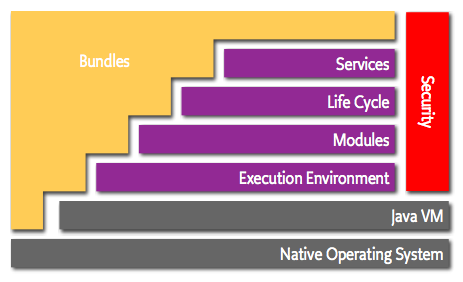
\includegraphics[width=0.73\textwidth]{layering-osgi.png}
\caption{\gls{OSGi} layered model \cite{OSGi}}
\label{fig:layering-osgi}
\end{figure}

\subsubsection{Implementations}
\gls{OSGi} is the foundation for many different Application Servers and IDEs. Some of the most widely used open source implementations of the \gls{OSGi} specification are listed here: 

\begin{itemize}
	\item \textbf{Eclipse Equinox} \\
		\url{http://eclipse.org/equinox/} \\
		Equinox is the core of the plug-in runtime for the Eclipse IDE.
	\item \textbf{Apache Felix} \\
		\url{http://felix.apache.org/} \\
		Apache Felix is the open source \gls{OSGi} implementation powered by the \gls{ASF} and is the basis of several other Apache projects like Apache Aries and Apache Karaf.
	\item \textbf{Knopflerfish} \\
		\url{http://www.knopflerfish.org/} \\
		Knopflerfish is the spin-off from one of the \gls{OSGi} alliance founding members and was open-sourced in 2003.
\end{itemize}

The developed framework uses Apache Felix for bundle testing purposes but aims to be \gls{OSGi} compliant and implementation independence. Apache Felix was chosen for its easy configuration and small memory footprint.

\subsection{Summary}
\gls{OSGi} is considered to be the most advanced module system for the Java platform. It supports all aspects of modularity, such as deployability, manageability, reusability and composability. Since modularity and its benefits and advantages, such as maintainability, is one of the main requirement of this work, \gls{OSGi} is the best choice as a foundation for the framework.

\fxfatal{Relates to my work how?}